\begin{minipage}{0.75\linewidth}
\begin{figure}[h]
    \centering
    \begin{adjustbox}{max width=1.0\linewidth, keepaspectratio}
        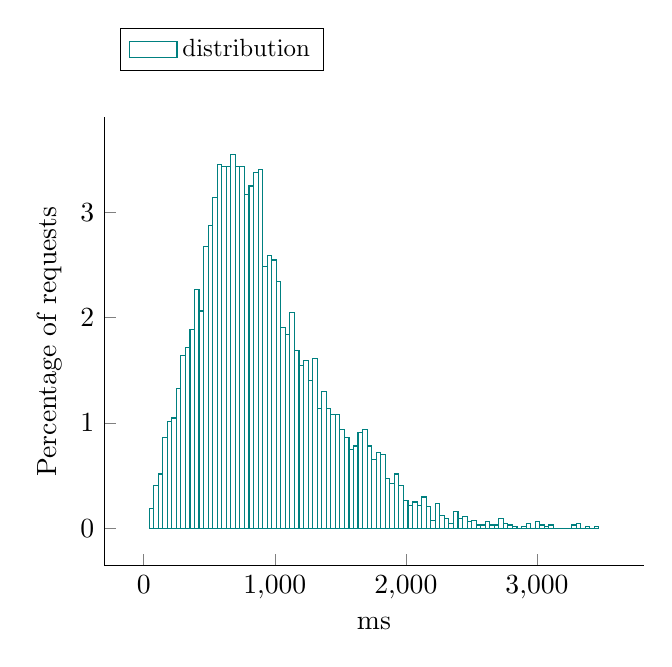
\begin{tikzpicture}
            \begin{axis}[ylabel = Percentage of requests, 
xlabel = ms, 
legend style = {nodes={scale=0.9, transform shape}, at={(0.03,1.2)}, anchor=north west, draw=black, fill=white, align=left, legend columns=3},
area style, mark size = 0pt,
 cycle list name = exotic,
  axis lines* = left]
		\addplot +[ybar interval] coordinates {
			 (41, 0.1875)
			 (75.65, 0.40625)
			 (110.3, 0.515625)
			 (144.95, 0.859375)
			 (179.6, 1.01562)
			 (214.25, 1.04688)
			 (248.9, 1.32812)
			 (283.55, 1.64062)
			 (318.2, 1.71875)
			 (352.85, 1.89062)
			 (387.5, 2.26562)
			 (422.15, 2.0625)
			 (456.8, 2.67188)
			 (491.45, 2.875)
			 (526.1, 3.14062)
			 (560.75, 3.45312)
			 (595.4, 3.4375)
			 (630.05, 3.4375)
			 (664.7, 3.54688)
			 (699.35, 3.4375)
			 (734, 3.4375)
			 (768.65, 3.17187)
			 (803.3, 3.25)
			 (837.95, 3.375)
			 (872.6, 3.40625)
			 (907.25, 2.48438)
			 (941.9, 2.59375)
			 (976.55, 2.54688)
			 (1011.2, 2.34375)
			 (1045.85, 1.90625)
			 (1080.5, 1.84375)
			 (1115.15, 2.04688)
			 (1149.8, 1.6875)
			 (1184.45, 1.54688)
			 (1219.1, 1.59375)
			 (1253.75, 1.40625)
			 (1288.4, 1.60938)
			 (1323.05, 1.14062)
			 (1357.7, 1.29688)
			 (1392.35, 1.14062)
			 (1427, 1.07812)
			 (1461.65, 1.07812)
			 (1496.3, 0.9375)
			 (1530.95, 0.859375)
			 (1565.6, 0.75)
			 (1600.25, 0.78125)
			 (1634.9, 0.90625)
			 (1669.55, 0.9375)
			 (1704.2, 0.78125)
			 (1738.85, 0.65625)
			 (1773.5, 0.71875)
			 (1808.15, 0.703125)
			 (1842.8, 0.46875)
			 (1877.45, 0.421875)
			 (1912.1, 0.515625)
			 (1946.75, 0.40625)
			 (1981.4, 0.265625)
			 (2016.05, 0.21875)
			 (2050.7, 0.25)
			 (2085.35, 0.21875)
			 (2120, 0.296875)
			 (2154.65, 0.203125)
			 (2189.3, 0.078125)
			 (2223.95, 0.234375)
			 (2258.6, 0.125)
			 (2293.25, 0.09375)
			 (2327.9, 0.046875)
			 (2362.55, 0.15625)
			 (2397.2, 0.09375)
			 (2431.85, 0.109375)
			 (2466.5, 0.0625)
			 (2501.15, 0.078125)
			 (2535.8, 0.03125)
			 (2570.45, 0.03125)
			 (2605.1, 0.0625)
			 (2639.75, 0.03125)
			 (2674.4, 0.03125)
			 (2709.05, 0.09375)
			 (2743.7, 0.046875)
			 (2778.35, 0.03125)
			 (2813, 0.015625)
			 (2847.65, 0)
			 (2882.3, 0.015625)
			 (2916.95, 0.046875)
			 (2951.6, 0)
			 (2986.25, 0.0625)
			 (3020.9, 0.03125)
			 (3055.55, 0.015625)
			 (3090.2, 0.03125)
			 (3124.85, 0)
			 (3159.5, 0)
			 (3194.15, 0)
			 (3228.8, 0)
			 (3263.45, 0.03125)
			 (3298.1, 0.046875)
			 (3332.75, 0)
			 (3367.4, 0.015625)
			 (3402.05, 0)
			 (3436.7, 0.015625)
			 (3471.35, 0)
		};
\addlegendentry{distribution};
           \end{axis}
      \end{tikzpicture}
  \end{adjustbox}
  \caption{Response time distribution - req = ReadTimeline-2}
\end{figure}
\end{minipage}\hfill\begin{minipage}{0.18\linewidth}
\begin{table}[h]
\begin{tabular}{|cc|}
\hline
\textbf{} & \textbf{ms}\\ \hline
 \Xhline{0.005\arrayrulewidth}
min & 41\\
 \Xhline{0.005\arrayrulewidth}
max & 3506\\
 \Xhline{0.005\arrayrulewidth}
mean & 921\\
 \Xhline{0.005\arrayrulewidth}
std & 493\\
\hline
\hline
 \Xhline{0.005\arrayrulewidth}
25th & 575\\
 \Xhline{0.005\arrayrulewidth}
50th & 828\\
 \Xhline{0.005\arrayrulewidth}
75th & 1184\\
 \Xhline{0.005\arrayrulewidth}
80th & 1299\\
 \Xhline{0.005\arrayrulewidth}
85th & 1435\\
 \Xhline{0.005\arrayrulewidth}
90th & 1623\\
 \Xhline{0.005\arrayrulewidth}
95th & 1848\\
 \Xhline{0.005\arrayrulewidth}
99th & 2411\\
\hline
\end{tabular}
\caption{Response time}
\end{table}
\end{minipage}\hfill